\documentclass[11pt]{article}
\usepackage[a4paper,total={6in,8in},margin=1in]{geometry}
\geometry{letterpaper}
\usepackage[utf8]{inputenc} % allow utf-8 input
\usepackage[T1]{fontenc}    % use 8-bit T1 fonts
\usepackage{microtype,inconsolata}
\usepackage{times,latexsym}
\usepackage{graphicx}
\usepackage{subfig}
\usepackage{amsmath,amssymb,mathabx,mathtools,amsthm,nicefrac}
\usepackage[linesnumbered,ruled,vlined]{algorithm2e}
\usepackage{enumitem}
\usepackage[pagebackref,breaklinks,colorlinks]{hyperref}
\usepackage[skip=3pt,font=small]{subcaption}
\usepackage[skip=3pt,font=small]{caption}
\usepackage[dvipsnames,svgnames,x11names,table]{xcolor}
\usepackage[capitalise,noabbrev,nameinlink]{cleveref}
\usepackage{booktabs,tabularx,colortbl,multirow,multicol,array,makecell,tabularray}
\usepackage[english]{babel}
\usepackage{listings}

\definecolor{color-C00000}{rgb}{0.75,0,0}
\definecolor{red}{rgb}{1,0,0}

\def\E{{\rm E}}
\def\Var{{\rm Var}}
\def\I{{\bf I}}
\def\w{{\bf w}}
\def\B{{\bf B}}
\def\b{{\bf b}}
\def\a{\alpha}
\def\tI{\tilde{\bf I}}
\def\tM{\tilde{M}}

\def\bF{{\bar{F}}}
\def\F{{\bf F}}

\def\D{{\cal D}}
\def\C{{\cal C}}
\def\S{{\cal S}}
\def\L{{\cal L}}

\def\obs{{\rm obs}}
\def\syn{{\rm syn}}

\begin{document}

\begin{center}
{\bf\Large Computer Vision I: Project 5 (10 points)}

\vspace{1em}
Due on Dec. 31th, 11:59pm
\end{center}

\section{Background} 

This project is based on \textbf{Section 11.2.3: Learning by alternating back-propagation}. Read the textbook for more information.

\subsection{Objective}
The objective of this project is to experience the multi-layered generator network, which is a top-down generative model. It is a nonlinear generalization of the factor analysis model. This top-down generative model has the following properties:
\begin{enumerate}[leftmargin=*,nolistsep]
    \item Embedding. The model embeds the high-dimensional non-Euclidean manifold formed by the observed examples into the low-dimensional Euclidean space of the latent factors so that linear interpolation in the low-dimensional factor space results in nonlinear interpolation in the data space.
    \item Analysis. The model disentangles the variations in the observed examples into independent variations of latent factors.
    \item Synthesis. In contrast to the bottom-up descriptive model which samples in high-dimensional space to synthesize examples, the top-down model can synthesize new examples by sampling the factors from the known low-dimensional prior distribution and transforming the factors into the synthesized examples.
\end{enumerate}

\subsection{Python Library}

Please install the latest matplotlib, numpy, pillow, torch and torchvision. You are also welcome to utilize any libraries of your choice, \textbf{but please report them in your report (for autograder)!}
\color{red}
\textbf{Again, report any customized library in the report (do not go too crazy as this will add a significant burden to TAs).}
\color{black}

\subsection{What to hand in?}

Please submit both a formal report and the accompanying code. For the report, kindly provide a PDF version. You may opt to compose a new report or complete the designated sections within this document, as can be started by simply loading the tex file to Overleaf. Your score will be based on the quality of \textbf{your results}, \textbf{the analysis} (diagnostics of issues and comparisons) in your report, and your \textbf{code implementation}. You may delete all the images before handing them in, as they may be too large for the autograder.

\paragraph{Notice.} Do not modify the function names, parameters, and returns in the given code, unless explicitly specified in this document.

\subsection{Help}

Make a diligent effort to address any encountered issues independently, and in cases where challenges exceed your capabilities, do not hesitate to seek assistance! Collaboration with your peers is permitted, but it is crucial that you refrain from directly \textcolor{red}{examining or copying one another's code.}  Please be aware that you'll fail the course if our \textbf{code similarity checker}, which has found some prohibited behaviors before, detects these violations. For details, please refer to: \url{https://yzhu.io/s/teaching/plagiarism}.

\clearpage

\section{Introduction to the Deep Generative Model}
Notations. Let $\I$ be a $D$-dimensional observed example, such as an image. Let $z$ be the $d$-dimensional vector of continuous latent factors, $z  = (z_k, k = 1, ..., d)$. The traditional factor analysis model is $\I = W z + \epsilon$, where $W$ is $D \times d$ matrix, $\epsilon$ is a $D$-dimensional error vector or the observational noise, usually $d < D$, $z \sim {\rm N}(0, I_d)$, and $\epsilon \sim {\rm N}(0, \sigma^2 I_D)$. The deep generative model generalizes the linear mapping $W z$ to a non-linear mapping $g(z; \theta)$, where $g$ is a ConvNet, and $\theta$ collects all the connection weights and bias terms of the ConvNet. Then the model becomes \begin{eqnarray}
&&\I = g(z; \theta) + \epsilon, \nonumber \\
&&z \sim {\rm N}(0,  I_d), \; \epsilon \sim {\rm N}(0, \sigma^2 I_D), \; d < D.
\label{eq:ConvNetFA}
\end{eqnarray}
The reconstruction error is  $ \| \I - g(z; \theta) \|^2$.

Although $g(z; \theta)$ can be any nonlinear mapping, the ConvNet parameterization of $g(z; \theta)$ makes it particularly close to the original factor analysis. Specifically, we can write the top-down ConvNet as follows:
\begin{eqnarray}
z^{(l-1)} = g_l(W_l z^{(l)} + b_l), \label{eq:Conv2}
\end{eqnarray}
where $g_l$ is element-wise nonlinearity at layer $l$, $W_l$ is the weight matrix, $b_l$ is the vector of bias terms at layer $l $, and $\theta = (W_l, b_l, l = 1, ..., L)$.  $z^{(0)} = g(z; \theta)$, and $z^{(L)} = z$. The top-down ConvNet (\ref{eq:Conv2}) can be considered a recursion of the original factor analysis model, where the factors at the layer $l-1$ are obtained by the linear superposition of the basis vectors or basis functions that are column vectors of $W_l$, with the factors at the layer $l$ serving as the coefficients of the linear superposition. 

We employ the alternating back-propagation algorithm for maximum likelihood learning of the generator network that iterates the following two steps:

(1) {\em  Inferential back-propagation}: For each training example,  infer the continuous latent factors by Langevin dynamics.

(2) {\em Learning back-propagation}: Update the parameters given the inferred latent factors by gradient descent.  

Specifically, the joint density is $p(z, \I; \theta) = p(z) p(\I|z; \theta)$, and
\begin{eqnarray}
\log p(z, \I; \theta) &=& - \frac{1}{2\sigma^2} \|\I - g(z; \theta)\|^2 - \frac{1}{2} \|z\|^2 + {\rm constant}, \label{eq:complete}
\end{eqnarray}
where the constant term is independent of $z$ and $\theta$.

For the training data $\{\I_i, i = 1, ..., n\}$, the generator model can be trained by maximizing the log-likelihood
\begin{eqnarray}
L(\theta) = \frac{1}{n}  \sum_{i=1}^{n} \log p(\I_i; \theta).
\end{eqnarray}


The gradient of $L(\theta)$ is obtained according to the following identity
\begin{align}
\frac{\partial}{\partial \theta} \log p(\I; \theta) = \E_{p(z|\I; \theta)} \left[ \frac{\partial}{\partial \theta} \log p(z, \I;  \theta)\right].  \label{eq:EM}
\end{align}
In general, the expectation in (\ref{eq:EM}) is analytically intractable and has to be approximated by MCMC that samples from the posterior $p(z|\I; \theta)$, such as the Langevin inference dynamics, which iterates
\begin{eqnarray}
z_{\tau + 1} = z_\tau + \frac{s^2 }{2}\frac{\partial}{\partial z}  \log p(z_\tau, \I;  \theta) + s e_\tau,  \label{eq:LangevinG}
\end{eqnarray}
where  $\tau$ indexes the time step, $s$ is the step size, and  $e_\tau$  denotes the noise term,  $e_\tau \sim {\rm N}(0, I_d)$. for each $z_i$, only a single copy of $z_i$ is sampled from $p(z_i|\I_i, \theta)$ by running a finite number of steps of Langevin dynamics starting from the current value of $z_i$, i.e., the warm start. With  $z_i$ sampled from  $p(z_i \mid \I_i, \theta)$ for each observation $\I_i$ by the Langevin inference process,  the Monte Carlo approximation to $L'(\theta)$ is
\begin{eqnarray}
L'(\theta) &\approx& \frac{1}{n}  \sum_{i=1}^{n} \frac{\partial}{\partial \theta} \log p(z_i, \I_i;  \theta) \nonumber \\
&=& \frac{1}{n}  \sum_{i=1}^{n} \frac{1}{\sigma^2} \left(\I_i - g(z_i; \theta)\right)\frac{\partial}{\partial \theta} g(z_i; \theta). \label{eq:learningG}
\end{eqnarray}
The updating of $\theta$ solves a nonlinear regression problem so that the learned $\theta$ enables better reconstruction of $\I_i$ by the inferred $z_i$.

\section{Experiment}
For the lion-tiger images, you will learn a generative model with $2$-$dim$ latent factor vector. To reduce the computational complexity, all images can be resized into the size of $128 \times 128$ pixels. 
\begin{figure}[h]
	\centering
	\setlength{\fboxrule}{1pt}
	\setlength{\fboxsep}{0cm}	
	\subfloat{
		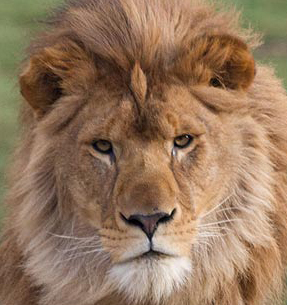
\includegraphics[width=.142\linewidth]{images/lion_1.jpg}
		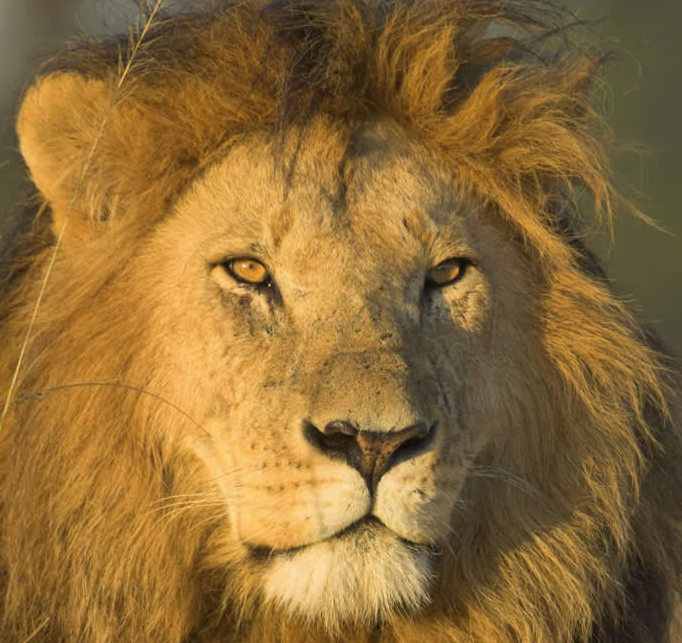
\includegraphics[width=.16\linewidth]{images/lion_2.jpg}
		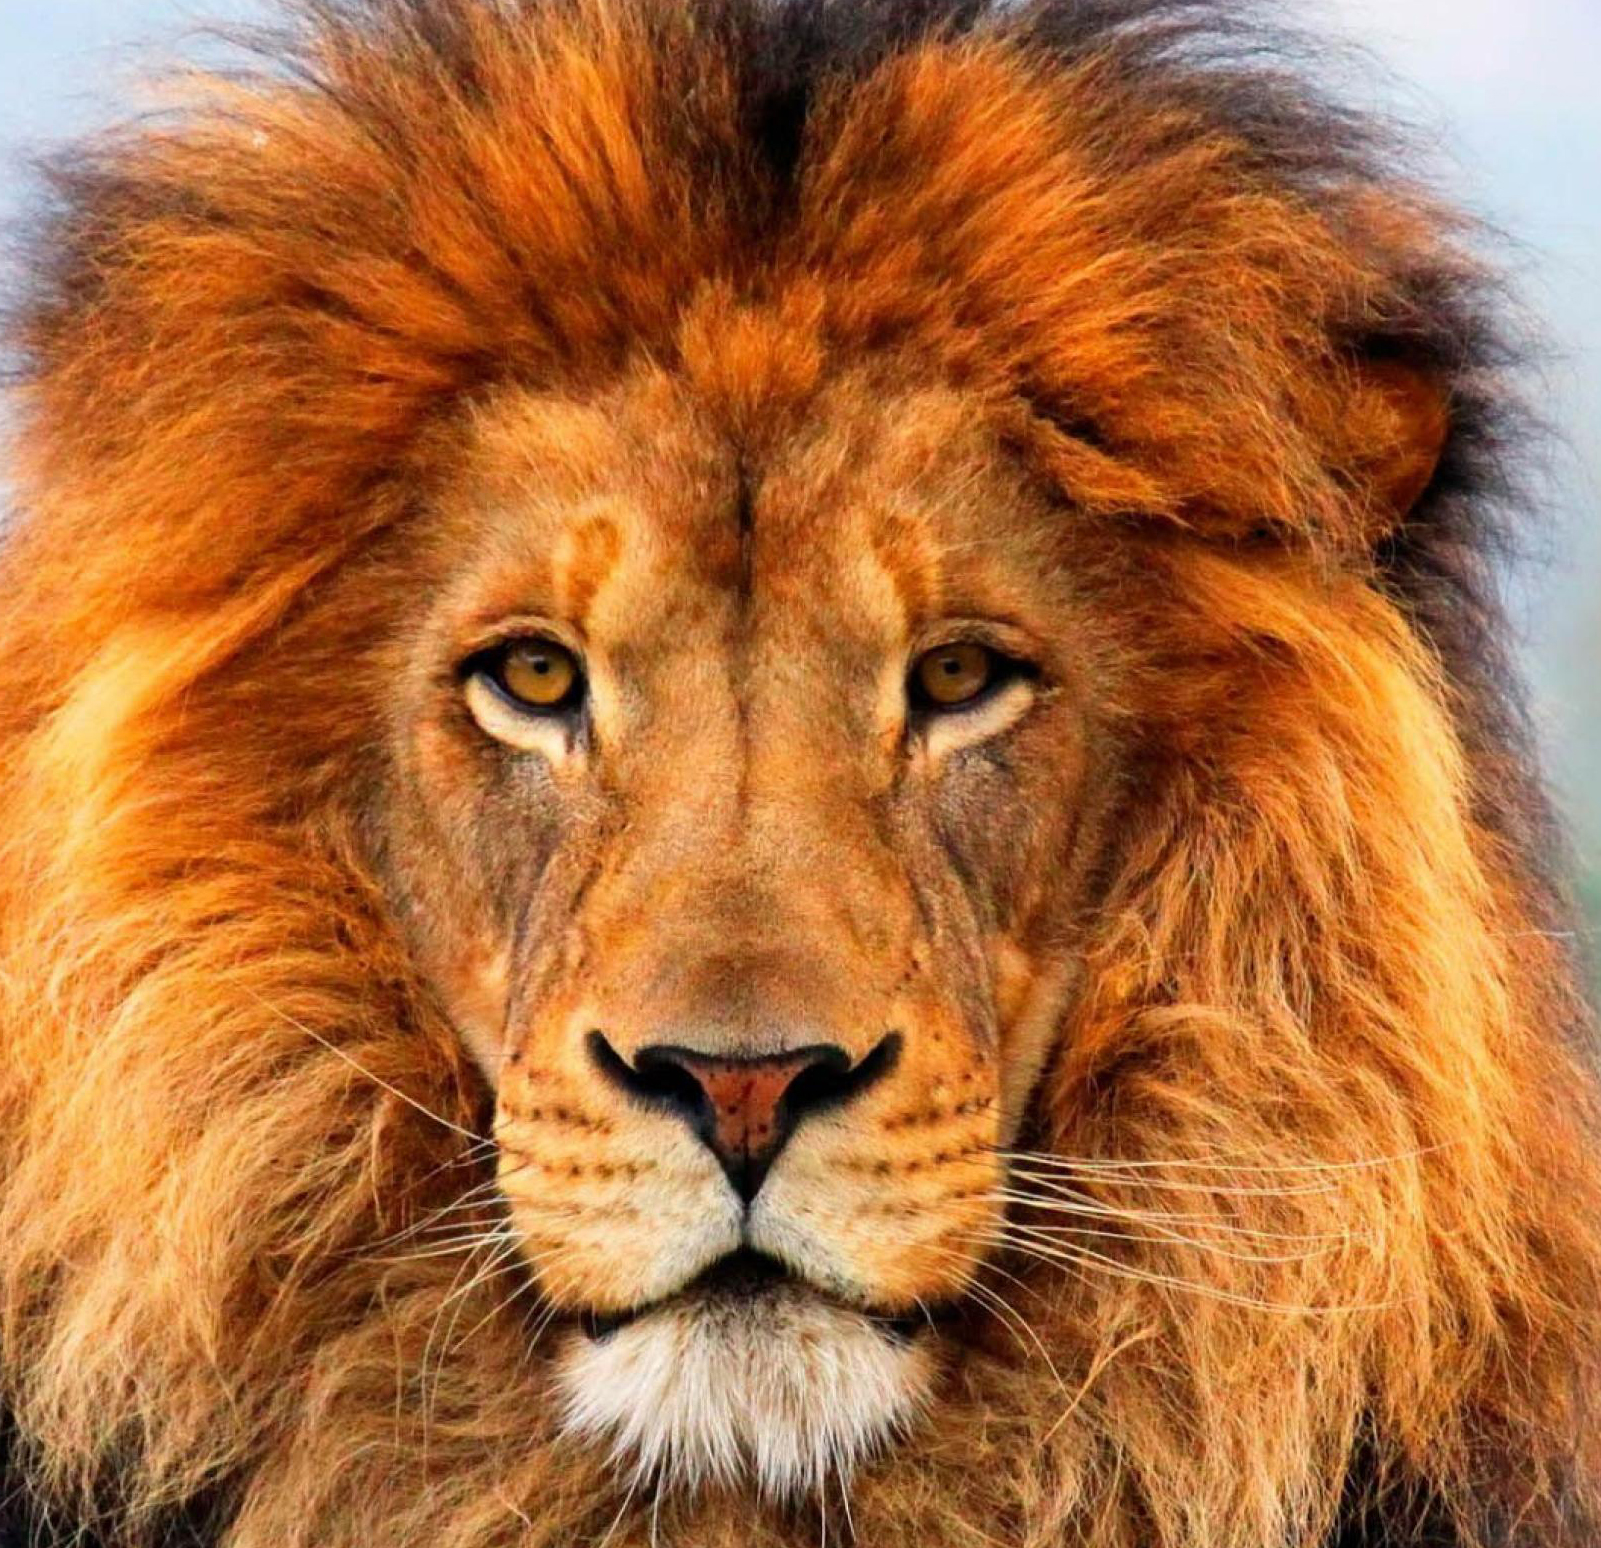
\includegraphics[width=.156\linewidth]{images/lion_3.jpg}
		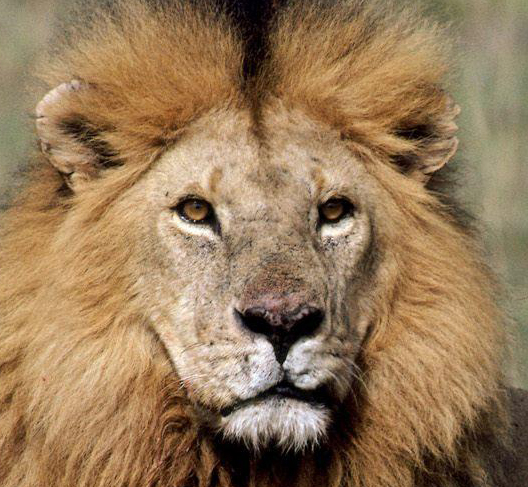
\includegraphics[width=.163\linewidth]{images/lion_4.jpg}
		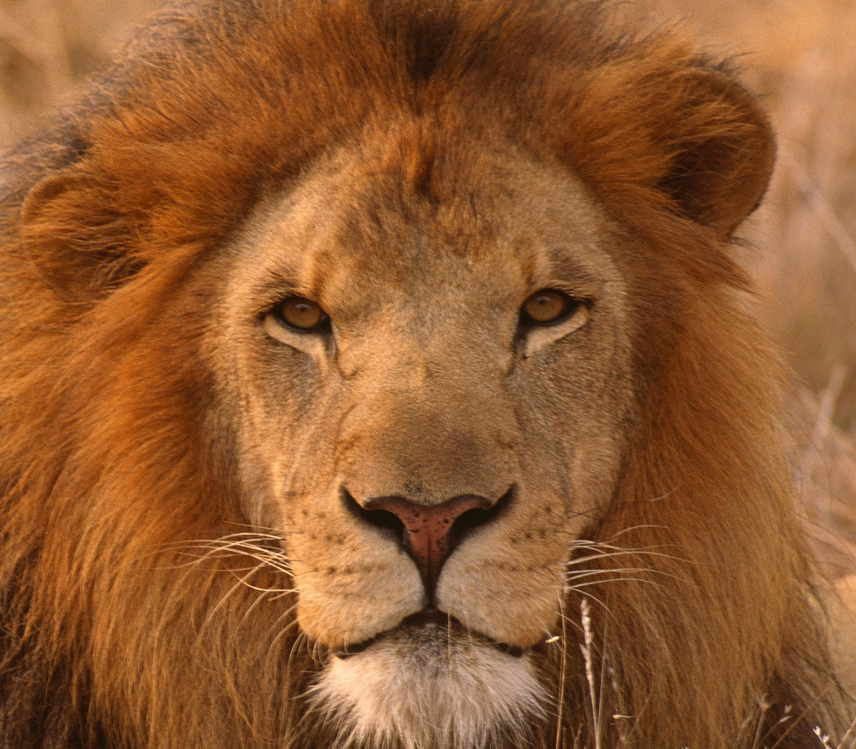
\includegraphics[width=.173\linewidth]{images/lion_5.jpg}
	}\\
    \subfloat{
    	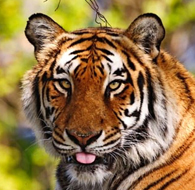
\includegraphics[width=.16\linewidth]{images/tiger_1.jpg}
    	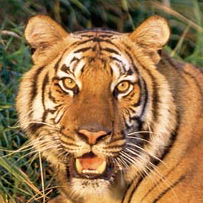
\includegraphics[width=.157\linewidth]{images/tiger_2.jpg}
    	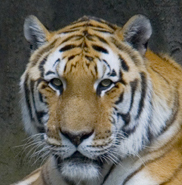
\includegraphics[width=.155\linewidth]{images/tiger_3.jpg}
    	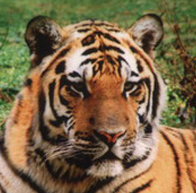
\includegraphics[width=.16\linewidth]{images/tiger_4.jpg}
    	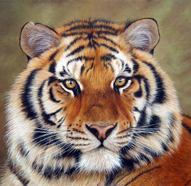
\includegraphics[width=.162\linewidth]{images/tiger_5.jpg}
    	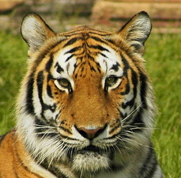
\includegraphics[width=.16\linewidth]{images/tiger_6.jpg}
    }\\[3px]
	\caption{lion-tiger images.}
\end{figure}

Fill the blank part of \texttt{abp.py}. Design your own structure of the generator. To generate vivid results, you should adjust the learning rate, discretization step size of the Langevin dynamics, the number of Langevin steps, and the annealing or tempering parameter $\sigma^2$ in Eq.\ref{eq:complete}.

\section{Submission}

(1) Reconstructed images of training images, using the inferred z from training images. Try both the warm-start scheme (running a finite number of steps of Langevin dynamics starting from the current value of $z_i$) and cold-start scheme (running a finite number of steps of Langevin dynamics starting from the fixed prior distribution of the latent factors)
\\~\\
(2) Randomly generated images, using randomly sampled z.
\\~\\
(3) Generated images with linearly interpolated latent factors from (-d, d).
For example, you interpolate 12 points from (-d, d) for each z dimension. Then you
will get a $12 \times 12$ panel of images. Determine the reasonable range (-d, d), and you should be able to see that tigers slightly change to lions.
\\~\\
(4) Plot of loss over iteration.
\\~\\
Write a report to show your results. And zip the report with your code.


\end{document}
